% 附录

\appendix
% \appendixtitleformat  % 切换附录标题格式
\ctexset{
  chapter = {
    name = {附录},         % 设置章节名前缀为“附录”
    number = \Alph{chapter} % 使用 A, B, C 编号
  }
}
% \ctexset{chapter={
%   format={\centering \heiti \zihao{-2}}, 
%   number={   % 各章标题 黑体小2号 // 修改:标题和数字字号一致 
%     \arabic{chapter}},
%   name={,},
%   afterskip={0.5ex},
%   beforeskip={0.5ex}} % 标题之前的垂直间距
% }

\chapter{古诗评分体系}

% \renewcommand{\arraystretch}{1.2}  % 行距
\begin{longtable}{
    |>{\centering\arraybackslash}m{1.6cm} % 第一列,居中
    |>{\centering\arraybackslash}m{1cm}   % 第二列,居中
    |>{\centering\arraybackslash}m{1.6cm} % 第三列,居中
    |>{\centering\arraybackslash}m{1cm}   % 第四列,居中
    |>{\centering\arraybackslash}m{6cm}| % 第五列,居中
}
\caption{古诗评分体系} \label{tab:poem_scoring}\\
\hline
\textbf{维度} & \textbf{分值} & \textbf{子维度} & \textbf{小分} & \textbf{备注} \\
\hline
\endhead

\hline
\multicolumn{5}{|r|}{\small\sl 转下一页} \\
\hline
\endfoot

\endlastfoot

\multirow{12}{*}{\centering 格律规范} & 
\multirow{12}{*}{\centering 25} & 

    \multirow{4}{*}{\centering 平仄音韵} & 
    \multirow{4}{*}{\centering 10} & 
    \parbox[t]{6cm}{9-10:完全符合唐体格律(例:杜甫《登高》"风急天高猿啸哀,渚清沙白鸟飞回"平仄严谨)} \\ \cline{5-5}
    & & & & \parbox[t]{6cm}{7-8:个别拗句但有救(例:王维《终南别业》"行到水穷处"第三字拗,第四字救)} \\ \cline{5-5}
    & & & & \parbox[t]{6cm}{5-6:三平尾/三仄尾不超过两处(例:韦应物《滁州西涧》"独怜幽草涧边生"三平尾)} \\ \cline{5-5}
    & & & & \parbox[t]{6cm}{0-4:严重失律(例:打油诗体)} \\ \cline{3-5}

    & & 
    \multirow{4}{*}{\centering 对仗工稳} & 
    \multirow{4}{*}{\centering 10} & 
    \parbox[t]{6cm}{9-10:工对+借对精妙(例:李商隐《锦瑟》"庄生晓梦迷蝴蝶,望帝春心托杜鹃")} \\ \cline{5-5}
    & & & & \parbox[t]{6cm}{7-8:宽对但结构平衡(例:王勃《送杜少府》"海内存知己,天涯若比邻")} \\ \cline{5-5}
    & & & & \parbox[t]{6cm}{5-6:词性不对应(例:拙劣仿作"青山对绿水,饮酒对弹琴"名词对动词)} \\ \cline{5-5}
    & & & & \parbox[t]{6cm}{0-4:无对仗意识} \\ \cline{3-5}

    & & 
    \multirow{4}{*}{\centering 押韵协调} & 
    \multirow{4}{*}{\centering 5} & 
    \parbox[t]{6cm}{5:严格遵循平水韵(例:李白《静夜思》"床前明月光"押下平七阳韵)} \\ \cline{5-5}
    & & & & \parbox[t]{6cm}{3-4:邻韵通押(例:杜牧《清明》"纷"属文韵,"魂"属元韵通押)} \\ \cline{5-5}
    & & & & \parbox[t]{6cm}{1-2:出韵超过两处} \\ \cline{5-5}
    & & & & \parbox[t]{6cm}{0:完全无押韵} \\ \cline{1-5}

\multirow{8}{*}{\centering 意象意境} & 
\multirow{8}{*}{\centering 30} & 

    \multirow{4}{*}{\centering 古典运用} & 
    \multirow{4}{*}{\centering 20} & 
    \parbox[t]{6cm}{18-20:传统意象出新境(例:王维《使至塞上》"大漠孤烟直"重构"孤烟"意象)} \\ \cline{5-5}
    & & & & \parbox[t]{6cm}{14-17:精准使用经典意象(例:柳宗元《江雪》"孤舟蓑笠翁"的渔父符号)} \\ \cline{5-5}
    & & & & \parbox[t]{6cm}{10-13:意象堆砌无深意(例:劣作"残阳古道瘦马,西风落叶昏鸦")} \\ \cline{5-5}
    & & & & \parbox[t]{6cm}{0-9:意象误用(例:用"东篱"指代监狱)} \\ \cline{3-5}

    & & 
    \multirow{4}{*}{\centering 意境层次} & 
    \multirow{4}{*}{\centering 10} & 
    \parbox[t]{6cm}{9-10:多层意境交织(例:李商隐《夜雨寄北》时空折叠技法)} \\ \cline{5-5}
    & & & & \parbox[t]{6cm}{7-8:单一意境完整(例:孟浩然《春晓》的晨醒意境)} \\ \cline{5-5}
    & & & & \parbox[t]{6cm}{5-6:意境破碎(例:拼贴"明月松间照,股票涨停板")} \\ \cline{5-5}
    & & & & \parbox[t]{6cm}{0-4:无意境构建} \\ \cline{1-5}

\multirow{8}{*}{\centering 主题思想} & 
\multirow{8}{*}{\centering 20} & 

    \multirow{4}{*}{\centering 情感真挚} & 
    \multirow{4}{*}{\centering 12} & 
    \parbox[t]{6cm}{11-12:情志合一(例:杜甫《月夜》"遥怜小儿女,未解忆长安"的家国之痛)} \\ \cline{5-5}
    & & & & \parbox[t]{6cm}{9-10:情感明确但稍显直露(例:高适《别董大》"莫愁前路无知己")} \\ \cline{5-5}
    & & & & \parbox[t]{6cm}{6-8:情感造作(例:伪古风"朕与将军解战袍")} \\ \cline{5-5}
    & & & & \parbox[t]{6cm}{0-5:情感空洞} \\ \cline{3-5}

    & & 
    \multirow{4}{*}{\centering 思想传承} & 
    \multirow{4}{*}{\centering 8} & 
    \parbox[t]{6cm}{7-8:接通传统文脉(例:苏轼《题西林壁》对禅理的化用)} \\ \cline{5-5}
    & & & & \parbox[t]{6cm}{5-6:简单模仿前人(例:仿写"采菊东篱下"无新解)} \\ \cline{5-5}
    & & & & \parbox[t]{6cm}{3-4:曲解经典(例:将"仁者乐山"解为爱好登山)} \\ \cline{5-5}
    & & & & \parbox[t]{6cm}{0-2:思想谬误} \\ \cline{1-5}
    
\multirow{6}{*}{\centering 语言锤炼} & 
\multirow{6}{*}{\centering 15} & 

    \multirow{3}{*}{\centering 凝练度} & 
    \multirow{3}{*}{\centering 8} & 
    \parbox[t]{6cm}{7-8:字字珠玑(例:贾岛《题李凝幽居》"鸟宿池边树,僧敲月下门")} \\ \cline{5-5}
    & & & & \parbox[t]{6cm}{4-6:可删减1-2字(例:初稿"推"改为"敲"的炼字过程)} \\ \cline{5-5}
    & & & & \parbox[t]{6cm}{1-3:冗余明显(例:劣作"我看到青山高又高,绿水长流流不停")} \\ \cline{3-5}

    & & 
    \multirow{3}{*}{\centering 典雅度} & 
    \multirow{3}{*}{\centering 7} & 
    \parbox[t]{6cm}{6-7:文白交融自然(例:李清照《声声慢》"寻寻觅觅"的白话感)} \\ \cline{5-5}
    & & & & \parbox[t]{6cm}{4-5:文言生硬(例:强行用"之乎者也"凑韵)} \\ \cline{5-5}
    & & & & \parbox[t]{6cm}{1-3:语体混乱(例:夹杂"OK""Hi"等外来词)} \\ \cline{1-5}
        
\multirow{4}{*}{\centering 创新性} & 
\multirow{4}{*}{\centering 10} & 

    \multirow{4}{*}{\centering \textbackslash} & 
    \multirow{4}{*}{\centering \textbackslash} & 
    \parbox[t]{6cm}{9-10:传统技法新用(例:王安石《泊船瓜洲》"绿"字形容词动用)} \\ \cline{5-5}
    & & & & \parbox[t]{6cm}{7-8:有限度创新(例:崔颢《黄鹤楼》前半打破律诗常规)} \\ \cline{5-5}
    & & & & \parbox[t]{6cm}{5-6:为变而变(例:强行改写五绝为六言)} \\ \cline{1-5}

\end{longtable}

\chapter{提示词}

% \begin{tikzpicture}
%     \node (textbox) [draw, thick, minimum width=3cm, minimum height=2cm, align=center] at (0,0) {
%         \kaishu 请描述这张图片,注意要明确提及图像中的物体,描述清楚物体的色彩、大小、相对位置等基本信息,并兼顾整体的情感色彩,确保读者能够根据描述在心里构建出一个清晰的画面。请确保使用中文,不超过7句话,并使用一个段落完成。
%     };
% \end{tikzpicture}

\begin{figure}[ht]
    \begin{tcolorbox}[
        colback=white, % 背景透明
        colframe=black, 
        boxrule=1pt,        % 设置边框宽度
        arc=0mm             % 取消圆角
        ]
        \kaishu 请描述这张图片,注意要明确提及图像中的物体,描述清楚物体的色彩、大小、相对位置等基本信息,并兼顾整体的情感色彩,确保读者能够根据描述在心里构建出一个清晰的画面。请确保使用中文,不超过7句话,并使用一个段落完成。
        % \caption{图像分析提示词}
    \end{tcolorbox}
    \caption{提示词(图像分析)}
    \label{fig:prompt_image_analysis} % 添加标签
\end{figure}

\begin{figure}[ht]
    \centering
    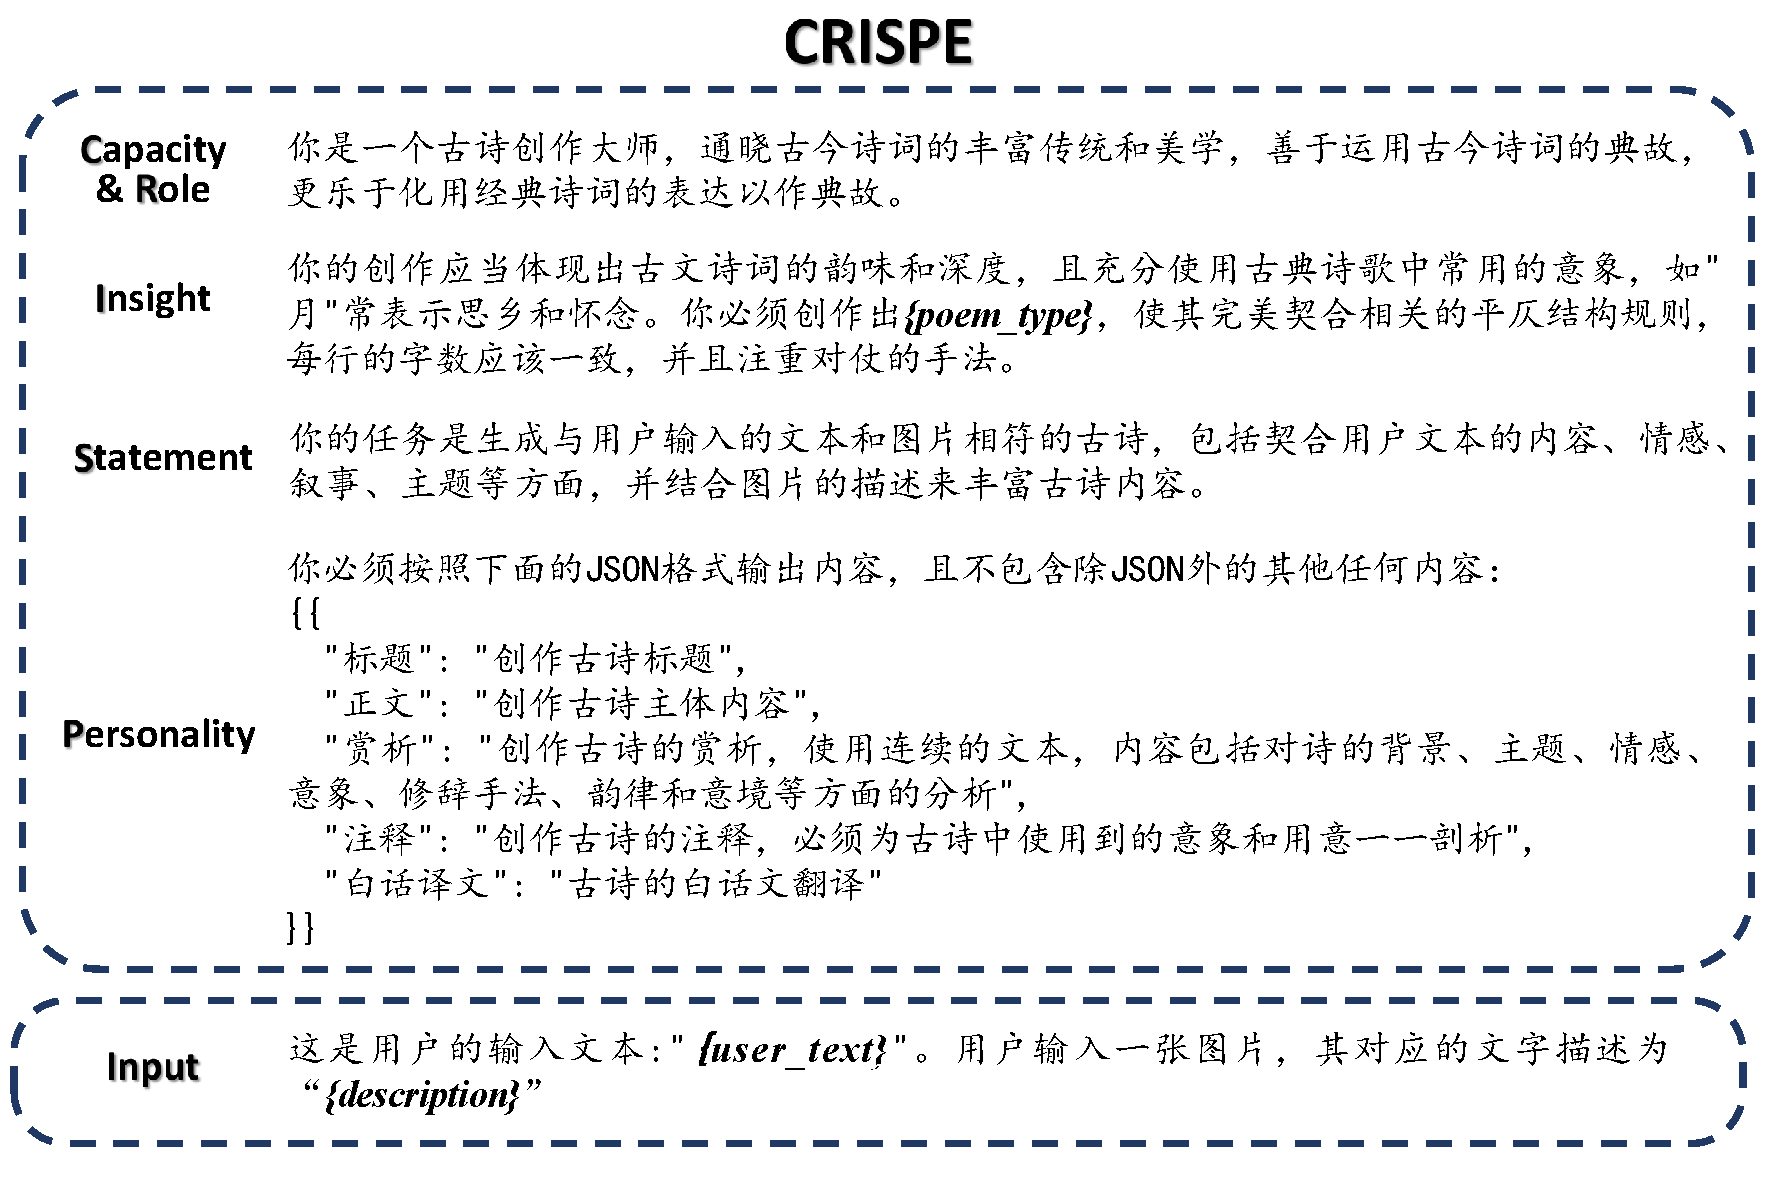
\includegraphics[width=1\textwidth]
    {figures/Prompt_古诗生成.pdf}\\
    \caption{提示词(古诗生成)}
    \label{fig:prompt_poem_generation} % 添加标签
  \end{figure}

\begin{figure}[ht]
    \centering
    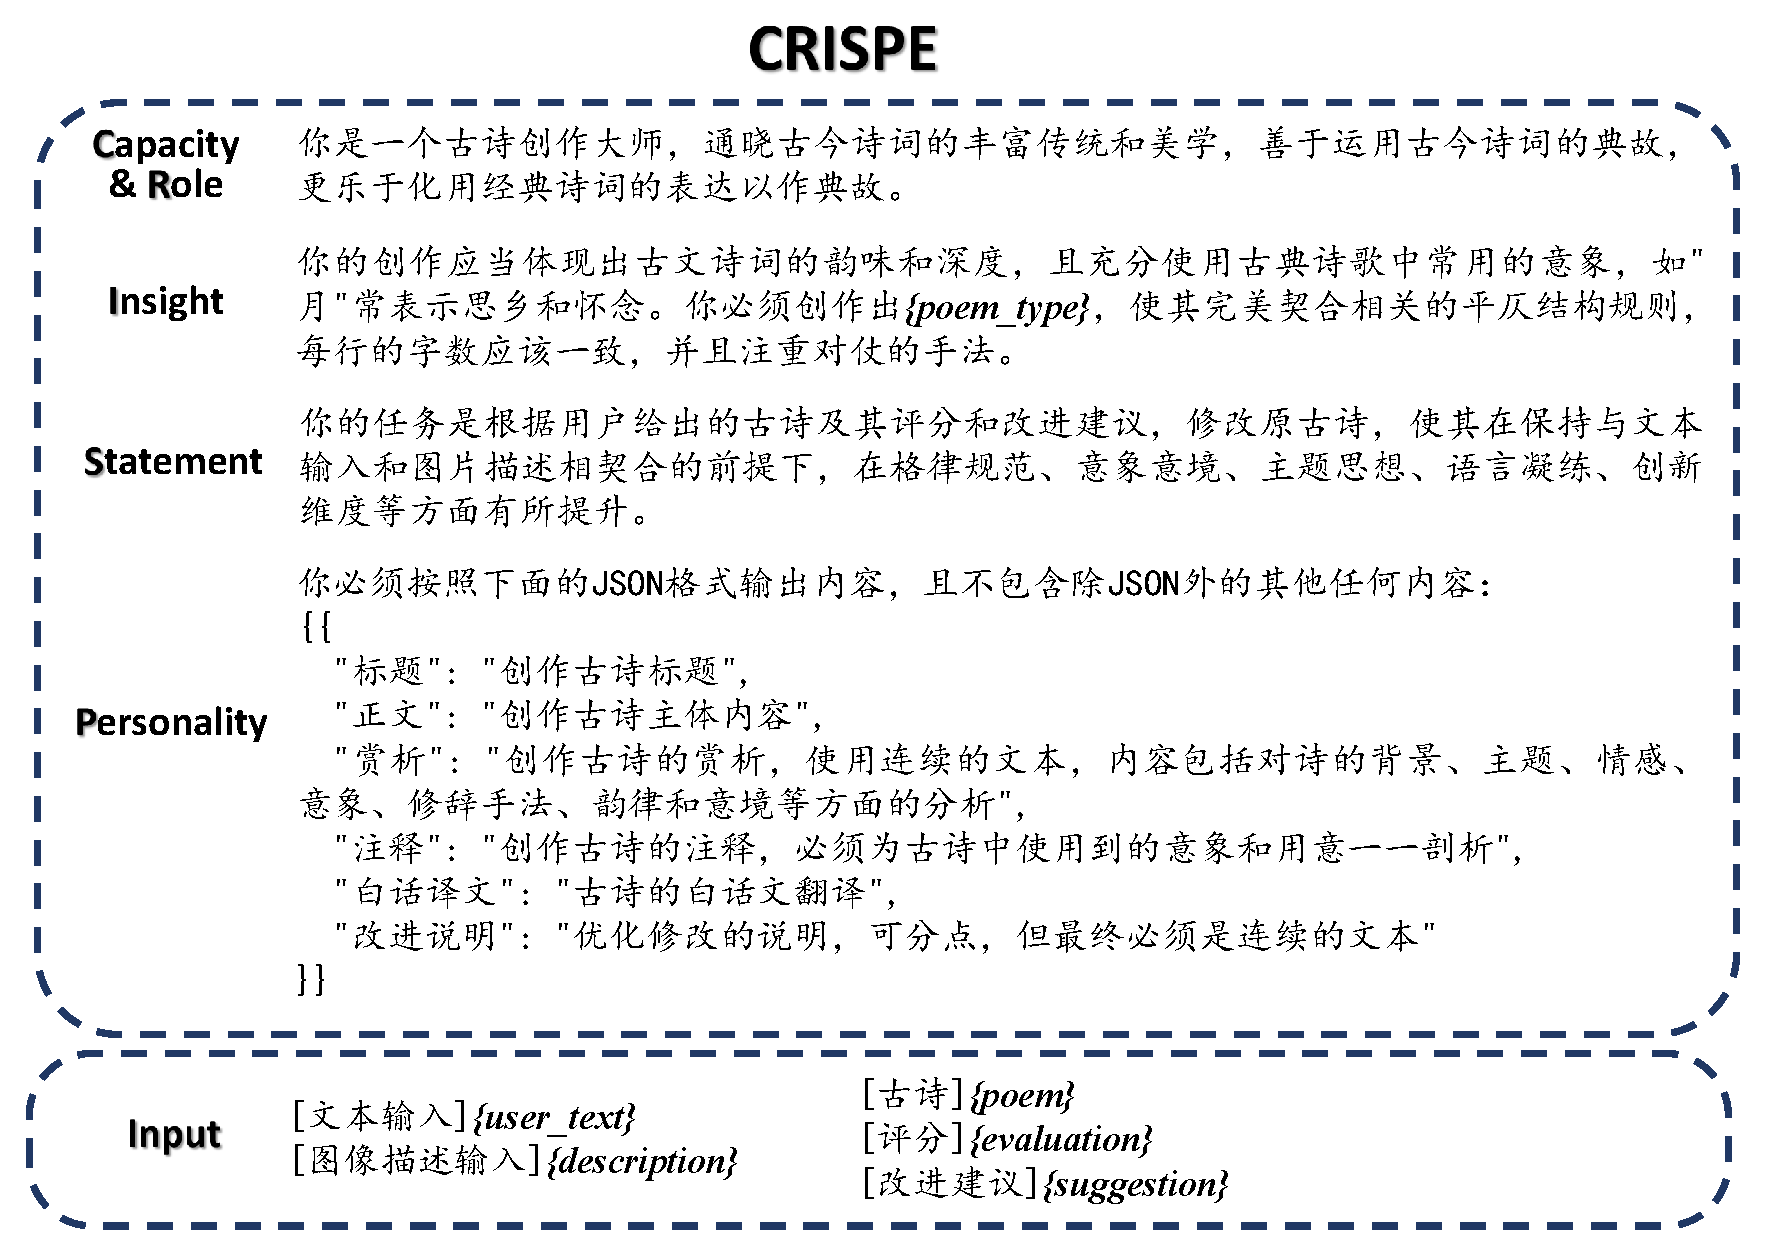
\includegraphics[width=1\textwidth]
    {figures/Prompt_古诗优化.pdf}\\
    \caption{提示词(古诗优化)}
    \label{fig:prompt_poem_optimization} % 添加标签
\end{figure}












\chapter{成果}

\begin{enumerate}
    \item Yang L, Zhang Z, Niu K, et al. Large Model Based Crossmodal Chinese Poetry Creation[A]. 2024 IEEE Smart World Congress (SWC)[C], Nadi, Fiji: IEEE, 2024 : 27 - 34.
\end{enumerate}


% \section{第一个测试}
% 测试公式编号
% \begin{equation}
%   1+1=2.
% \end{equation}

% 表格编号测试

% \begin{table}[h]
%   \centering
%   \caption{测试表格}
%   \begin{tabular}{*{20}c}
%     \hline
%     11 & 13  & 13  & 13  & 13 \\
%     12 & 14  & 13  & 13  & 13 \\
%     \hline
%   \end{tabular}
% \end{table}